\documentclass[conference]{IEEEtran}

\usepackage{graphicx}
\usepackage{float}
\usepackage{afterpage}
\usepackage{hyperref}
\usepackage{listings}
\usepackage{import}

%bib
\bibliographystyle{IEEEtran}

% correct bad hyphenation here
\hyphenation{op-tical net-works semi-conduc-tor}

% path to figures
\graphicspath{{figures/}}

%capshun space
%\setlength{\abovecaptionskip}{5pt plus 0pt minus 0pt}

\begin{document}
%
% paper title
% can use linebreaks \\ within to get better formatting as desired
\title{Web Application Model Generation \\through Reverse Engineering and UI Pattern Inferring}

% author names and affiliations
% use a multiple column layout for up to three different
% affiliations
\author{\IEEEauthorblockN{Clara Sacramento, Ana C. R. Paiva}
\IEEEauthorblockA{Departamento de Engenharia Informática\\
Faculdade de Engenharia da Universidade do Porto\\
Porto, Portugal\\
ei09090@fe.up.pt; apaiva@fe.up.pt; }}

% use for special paper notices
%\IEEEspecialpapernotice{(Invited Paper)}

% make the title area
\maketitle

\begin{abstract}
%\boldmath
A great deal of effort in model-based testing is related to the creation of the model. The model itself, while a powerful tool of abstraction, can be a source of bugs. This paper presents a dynamic reverse engineering approach that aims to extract part of the model of an existing Web application through the identification of User Interface (UI) patterns. This approach explores the Web application via crawling, saves information related to the interaction (crawl history, HTML pages and their URLs), analyzes the gathered information, and infers the UI patterns via a set of heuristics rules.
\end{abstract}
\begin{IEEEkeywords} Reverse Engineering, Web Application, UI Patterns, Web Scraping, Web Crawling \end{IEEEkeywords}

\IEEEpeerreviewmaketitle

\section{Introduction}\label{sec:intro}

Web applications are getting more and more important, and can now handle tasks that before could only be performed by desktop applications \cite{garrett2005ajax}, like editing images or creating spreadsheet documents. However, despite their growing relevance, they still suffer from a lack of standards and conventions \cite{constantine2002usage}, unlike desktop and mobile applications. This means that the same task can be implemented in many different ways, which makes automated Web application testing difficult to accomplish and inhibits reuse of testing code. 

Graphical User Interfaces of all kinds are populated with recurring behaviors that vary slightly, an example being authentication (\textit{login/password}). These behaviors (patterns) are called User Interface (UI) patterns \cite{van2001patterns} and are recurring solutions that solve common design problems. Due to their widespread use, UI patterns allow users a sense of familiarity and comfort when using applications. 

However, while UI patterns are familiar to users, their implementation may vary significantly. Even a simple pattern like authentication can be implemented in many ways. Authentication failure can trigger the appearance of an error message; but some implementations simply erase the inserted data, with no error message visible. Despite this, it is possible to define generic and reusable test strategies to test them after a configuration process to adapt the tests to those different possible applications \cite{morgado2012gui}. 

That is the main idea behind the PBGT (\textit{Pattern-based GUI Testing}) project, in which this research work is included. In the PBGT approach, the user builds a test model of the Web application with instantiations of UI patterns, and later uses that model to test the previous Web app.  The goal of the work described in this paper is to continue the work done in \cite{nabuco2013inferring} on the extraction process (PARADIGM-RE), and  its aim is to automatize the model process: visit a Web application automatically  via reverse engineering, search for UI patterns in its pages, and finally produce a model with the results of the search.

The rest of the paper is structured as follows. Section \ref{sec:intro} introduces this document, and resumes necessary background knowledge. Section \ref{sec:pbgt} presents an overview of the PBGT project, setting the context for this work. Section \ref{sec:sota} addresses the related work, as well as the tools available to perform the needed tasks. Section \ref{sec:re} describes the developed approach, its components and  their interrelations, and the results it produces. Section \ref{sec:eval} provides a practical example of the system proposed. Section \ref{sec:conc} provides the conclusions, reports some of the problems found and points out the future work. 

\section{PBGT Overview}\label{sec:pbgt}

As mentioned before, the focus of this article is a component of an investigation project named PBGT (\textit{Pattern-based GUI Testing}) \cite{moreira2013pattern}. The goal of this investigation project is to develop a model-based GUI testing tool and approach, usable as an industrial tool. 

\subsection{Architecture}
This project has five parts: a DSL (\textit{Domain Specific Language}) named \textbf{PARADIGM} to define GUI testing models based on UI patterns; \textbf{PARADIGM-RE}, a Web application reverse engineering tool whose purpose is to extract UI patterns from Web pages without access to their source code, and use the extracted patterns to generate a test model defined in PARADIGM; a modeling and testing environment, named \textbf{PARADIGM-ME}, made to support the creation of test models; an automatic test case generation tool, named \textbf{PARADIGM-TG}, that generates test cases from test models defined in PARADIGM; and finally a test case execution tool, named \textbf{PARADIGM-TE}, which executes test cases, analyzes their coverage, and returns detailed execution reports. The architecture and workflow of the project can better be seen in Fig. \ref{fig:pbgt}.

\begin{figure}[!htb]
\centering
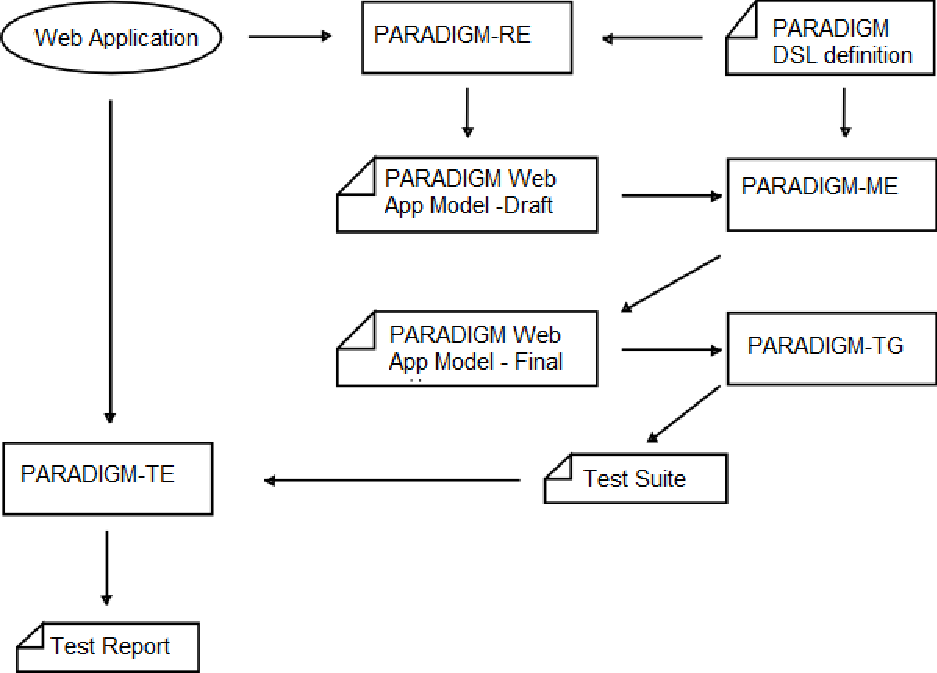
\includegraphics[width=0.45\textwidth]{pbgt}
\caption{An overview of the PBGT project}
\label{fig:pbgt}
\end{figure}

\subsection{Supported Patterns}
The UI Patterns defined in the PARADIGM language, and therefore supported by PARADIGM-RE, are:
\begin{description}
\item[\textit{Login}] \hfill \\
This pattern is commonly found in Web applications, especially in the ones that restrict access to functionalities or data. Usually consists of two input fields (a normal input box for email or username, and a cyphered text for the password) and a submit button, with optionally a ``remember me'' checkbox. The authentication process has two possible outcomes: valid and invalid.
\item[\textit{Search}] \hfill \\
This pattern consists of one or more input fields, where the user inserts keywords to search, and a submit button to start the search. The search may be submitted via a submit button, or dynamically upon text insertion. When the search is successful, the website shows a list of results; upon failure, an error message may be shown.
\item[\textit{Sort}] \hfill \\
This pattern sorts a list of data by a common attribute (price, name, relevance, etc.) according to a defined criteria (ascending or descending, alphabetically, etc.).
\item[\textit{Master Detail}] \hfill \\
This pattern is present in a webpage when selecting an element from a set (called \textit{master}) results in filtering/updating another related set (called \textit{detail}) accordingly. For example, clicking on a checkbox associated to a brand may include (or exclude) products of that brand in a product search result list. Generally the only elements changed are the elements belonging to the \textit{detail} set.
\item[\textit{Menu}] \hfill \\
This pattern is very common in webpages. It's usually defined as a tree structure with several navigational options, to provide easier access for users. 
\item[\textit{Input}] \hfill \\
This pattern is any kind of input field that allows the user to insert text.
\item[\textit{Call}] \hfill \\
This pattern is any kind of element where a click triggers a change of page.
\end{description}

\subsection{Produced Models}

The models produced by PARADIGM-RE after the RE process consist of a XML file that contains all the information about the UI Patterns found: their definition and configurations. The PARADIGM model generated by the PARADIGM-RE tool does not contain the connectors between the UI Patterns, only the UI Patterns and their configurations. These models are meant to be loaded to the PARADIGM-ME tool and completed manually.\\

\section{Reverse Engineering Approach}\label{sec:re}
The  approach described in this paper aims to improve on the previous work \cite{nabuco2013inferring} done on the PARADIGM-RE tool. The previous work extracted patterns from a

%uses a dynamic method to extract execution traces from which  additional information is inferred. An execution trace is the sequence of user actions executed during the interaction with a software system, such as clicks, text inputs and also some information of the system state (e.g., the information that is being displayed). 

\begin{figure}[!htb]
\centering
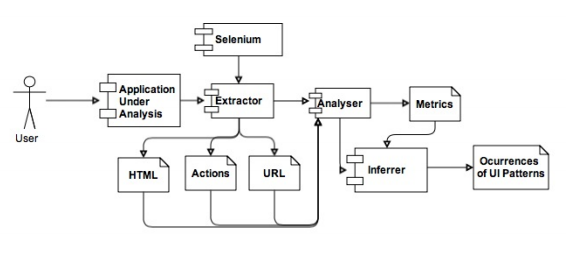
\includegraphics[width=0.45\textwidth]{retool}
\caption{The architecture of the PARADIGM-RE tool.}
\label{fig:retool}
\end{figure}

\subsection{File Processing}\label{sec:fp}

\subsection{UI Pattern Inferring}\label{sec:inf}

\section{Evaluation}\label{sec:eval}


\section{Related Work}\label{sec:sota}

Reverse engineering is ``the process of analyzing the subject system to identify the system components and interrelationships and to create representations of the system in another form or at a higher level of abstraction'' \cite{chikofsky1990reverse}. There are two methods of applying reverse engineering to a system: the dynamic method, in which the data are retrieved from the system at run time without access to the source code, the static method, which obtains the data from the system source code \cite{systa1999dynamic}, and finally the hybrid method, which combines the two previous methods \cite{canfora2011achievements}. These approaches follow the same main steps: collect the data, analyze it and represent it in a legible way, and in the process allow the discovery of information about the system's control and data flow \cite{pacione2003comparative}.

There are plenty of approaches that extract information from Web applications \cite{sampath2007applying,amalfitano2010rich, andjelkovic2011trace}. ReGUI \cite{coimbra2011reverse,coimbra2012dynamic} is a dynamic reverse engineering tool made to reduce the effort of modeling the structure and behavior of a software application GUI. Duarte, Kramer and Uchitel defined an approach for behavior model extraction which combines static and dynamic information \cite{duarte2006model}.

There are also plenty of approaches that crawl a Web application, and in the process extract information. Crawljax \cite{roest2010automated} is a tool that obtains graphical site maps by automatically crawling through a Web application. Mesbah \textit{et al.} proposed an approach named FeedEx \cite{fard2013feedback}, a feedback-directed Web application exploration technique to derive test models. It uses a greedy algorithm to partially crawl a RIA's GUI, and the goal is that the derived test model capture different aspects of the given Web application's client-side functionality. WebDiff \cite{choudhary2010Webdiff} is a tool that searches for cross-browser inconsistencies by analyzing a website's DOM and comparing screenshots obtained in different browsers. Dincturk \textit{et al.} \cite{dincturk2012statistical} proposed a RIA crawling strategy using a statistical model based on the model-based crawling approach introduced in \cite{benjamin2011strategy} to crawl RIAs efficiently. Dallmeier \textit{et al.}'s Webmate \cite{dallmeier2012Webmate,dallmeier2013Webmate} is a tool that analyzes the Web application under test, identifies all functionally different states, and is then able to navigate to each of these states at the user’s request.

User Interaction (UI) patterns, in particular the ones supported by the tool, are well-documented in a various number of sources \cite{tidwell2010designing,van2001patterns, neil12standard,sinnig2005patterns}. Lin and Landay's approach \cite{lin2008employing} uses UI patterns for Web applications that run on PCs and mobile phones, and prompt-and-response style voice interfaces. Pontico \textit{et al.}'s approach \cite{pontico2008organizing} presents UI patterns common in eGovernment applications.

Despite the fact that there are plenty of approaches to mine patterns from Web applications, no approaches have been found that infer UI patterns from Web applications beside the work extended in this paper \cite{nabuco2013inferring, morgado2012gui}. The approaches found deal mostly with Web mining, with the goal of finding relationships between different data or finding the same data in different formats. Brin \cite{brin1999extracting} presented an approach to extract relations and patterns for the same data spread through many different formats. Chang \cite{chang2003automatic} proposes a similar method to discover patterns, by extracting structured data from semi-structured Web documents.

\section{Conclusion}\label{sec:conc}
%The conclusion goes here.


\bibliography{bib}


% that's all folks
\end{document}


